%%%%%%%%%%%%%%%%%%%%%%%%%%%%%%%%%%%%%%%%%%%%%%%%%%%%
% Artifact Appendix Template for Usenix Security'24 AE
%%%%%%%%%%%%%%%%%%%%%%%%%%%%%%%%%%%%%%%%%%%%%%%%%%%%

\appendix
\section{Artifact Appendix}
% \textit{This artifact appendix is meant to be a self-contained document which
% describes a roadmap for the evaluation of your artifact. It should include a
% clear description of the hardware, software, and configuration requirements. In
% case your artifact aims to receive the functional or results reproduced badge,
% it should also include the major claims made by your paper and instructions on
% how to reproduce each claim through your artifact. Linking the claims of your
% paper to the artifact is a necessary step that ultimately allows artifact
% evaluators to reproduce your results.}

% \textit{Please fill all the mandatory sections, keeping their titles and
% organization but removing the current illustrative content, and remove the
% optional sections where those do not apply to your artifact.}

%%%%%%%%%%%%%%%%%%%%%%%%%%%%%%%%%%%%%%%%%%%%%%%%%%%%%%%%%%%%%%%%%%%%%
\subsection{Abstract}
% {\em [Mandatory]}
% {\em Provide a short description of your artifact.}

To defend DMA attacks effectively with low overhead, we design and implement \name, a novel hardware-software co-design to enforce spatial and temporal protection for DMA buffers. It registers information for each DMA buffer and signs the DMA pointers when creating DMA buffer mappings, and authenticates the DMA using the signature and corresponding buffer information, including a unique identifier and bounds.
\blfootnote{\Letter~Corresponding author.}
Before designing \name, we performed a detailed Characterization. We implemented \name on RISC-V and ARM QEMU, as well as on Rocket Chip based RISC-V SoC on FPGA.

This artifact contains the QEMU setup and analyzing tool to perform characterization, ARM and RISC-V QEMU with \name emulation, and FPGA-based SoC with \name and IOMMU hardware, as well as Linux kernels with corresponding drivers for each of the platforms described in implementation.

%%%%%%%%%%%%%%%%%%%%%%%%%%%%%%%%%%%%%%%%%%%%%%%%%%%%%%%%%%%%%%%%%%%%%
\subsection{Description \& Requirements}

% \textit{[Mandatory] This section should list all the information necessary to
% recreate the same experimental setup you have used to run your artifact. Where
% it applies, the minimal hardware and software requirements to run your artifact.
% It is also very good practice to list and describe in this section benchmarks
% where those are part of, or simply have been used to produce results with, your
% artifact.}
The private key and ssh configuration is provided in the HotCRP submission.

\subsubsection{Security, privacy, and ethical concerns}
% \textit{[Mandatory] Describe any risk for evaluators while executing your
% artifact to their machines security, data privacy or others ethical concerns.
% This is particularly important if destructive steps are taken or security
% mechanisms are disabled during the execution.}
None. But the reviewer may want to use VPN to connect to the provided server to avoid any potential information leakage.

\subsubsection{How to access}
% {\em [Mandatory]} \textit{Describe here how to access your artifact. If you are
% applying for the Artifacts Available badge, the archived copy of the artifacts
% must be accessible via a stable reference or DOI. For this purpose, we recommend
% Zenodo, but other valid hosting options include institutional and
% third-party digital repositories (e.g., FigShare, Dryad, Software
% Heritage, GitHub, or GitLab — not personal webpages). For repositories that can
% evolve over time (e.g., GitHub), a stable reference to the evaluated version
% (e.g., a URL pointing to a commit hash or tag) rather than the evolving version
% reference (e.g., a URL pointing to a mere repository) is required. Note that the
% stable reference provided at submission time is for the purpose of Artifact
% Evaluation. Since the artifact can potentially evolve during the evaluation to
% address feedback from the reviewers, another (potentially different) stable
% reference will be later collected for the final version of the artifact (to be
% included here for the camera-ready version).}
The DOI is \code{10.5281/zenodo.12216074}.
It can be accessed via \url{https://doi.org/10.5281/zenodo.12216074}.
All the required copy of the files are contained in \code{/home/reviewer/Artifacts} in the provided server.
Reviewers may want to use the local version directly since the artifacts is quite large.


\subsubsection{Hardware dependencies}
% {\em [Mandatory]} \textit{Describe any specific hardware features required to
% evaluate your artifact (vendor, CPU/GPU/FPGA, number of processors/cores,
% microarchitecture, interconnect, memory, hardware counters, etc). If your
% artifact requires special hardware, please provide instructions on how to gain
% access to the hardware. For example, provide private SSH keys to access the
% machines remotely. Please keep in mind that the anonymity of the reviewers needs
% to be maintained and you may not collect or request personally identifying
% information (e.g., email, name, address). [Simply write "None." where this does
% not apply to your artifact.]}

The provided server is already connected to the hardware.

XCKU040 FPGA, FMC-to-PCIe adaptor card, SD card, PCIe device required to test the functionality of the SoC with DMAAUTH support.

\begin{figure}[!h]
    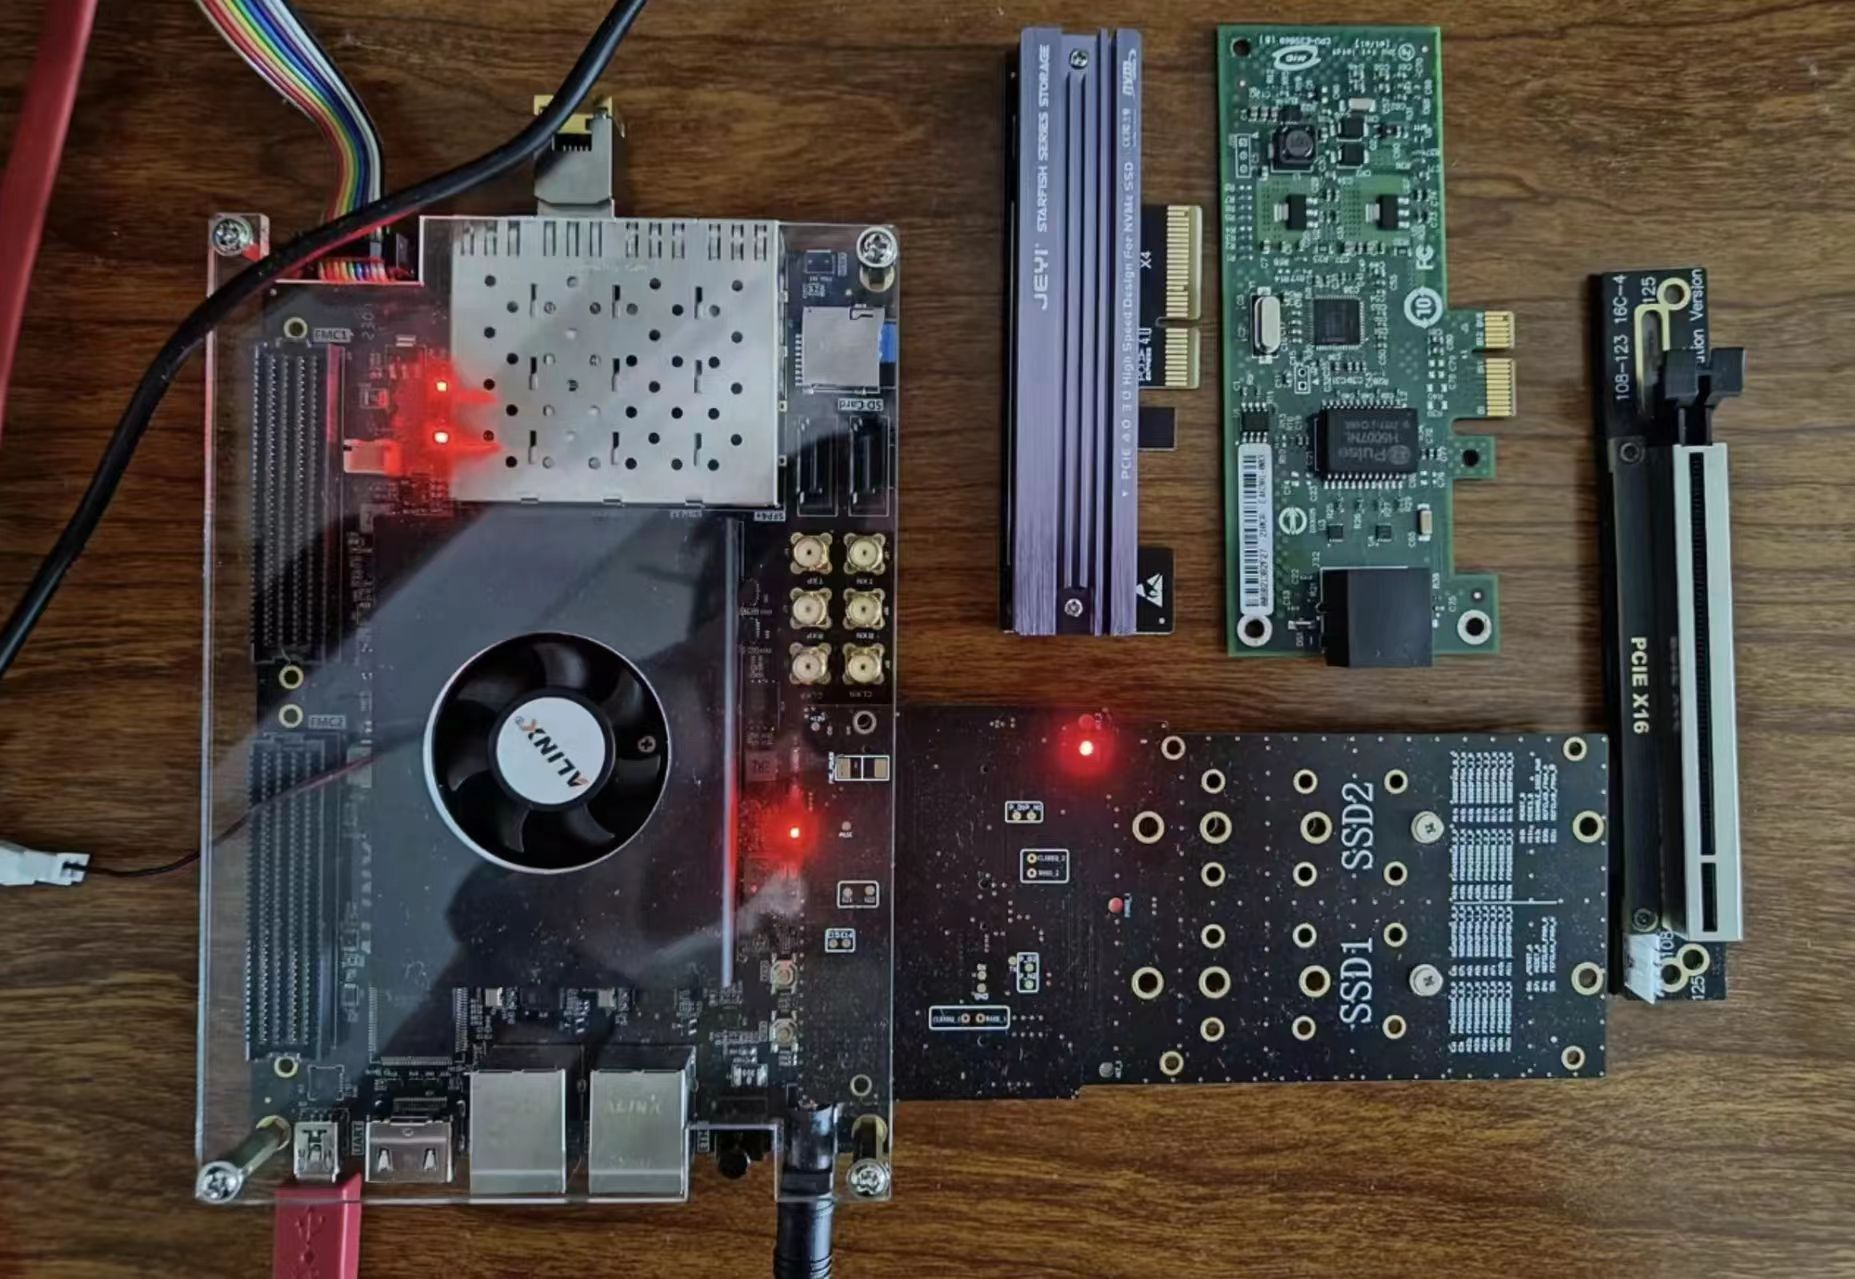
\includegraphics[width=\linewidth]{figures/platform.jpg}
    \caption{Hardware platform for the artifacts.}
\end{figure}


\subsubsection{Software dependencies}
% {\em [Mandatory]} \textit{Describe any specific OS and software packages
% required to evaluate your artifact. This is particularly important if you share
% your source code and it must be compiled or if you rely on some proprietary
% software that you cannot include in your package. In such a case, you must
% describe how to obtain and to install all third-party software, data sets, and
% models. [Simply write "None." where this does not apply to your artifact.]}
The provided server is already capable of running the artifact. The environment is Ubuntu 22.04.4 LTS with the required package to build Linux kernel, and AMD Vivado 2022.02.

\subsubsection{Benchmarks}
% {\em [Mandatory]} \textit{Describe here any data (e.g., data-sets, models,
% workloads, etc.) required by the experiments with this artifact reported in your
% paper.} \textit{[Simply write "None." where this does not apply to your
% artifact.]}
None.

%%%%%%%%%%%%%%%%%%%%%%%%%%%%%%%%%%%%%%%%%%%%%%%%%%%%%%%%%%%%%%%%%%%%%
\subsection{Set-up}

% {\em [Mandatory]} \textit{This section should include all the installation and
% configuration steps required to prepare the environment to be used for the
% evaluation of your artifact.}

The environment is already provided on the server. If using our provided server, skip the A.3.1 section.

For reviewers who want to try the artifact on their own machine, the following steps are required.

1. Please install the dependencies required to build the Linux kernel. 2. Please install Vivado 2022.2 to build the FPGA bitstream. 3. Download and extract the artifacts from provided zenodo DOI.

\subsubsection{Installation}
% {\em [Mandatory]} \textit{Instructions to download and install dependencies as
% well as the main artifact. After these steps the evaluator should be able to run
% a simple functionality test.}
If using the provided server, no extra steps are required.

When evaluating the artifacts on your local machine, about 300GB of disk space is required. And we recommend using Ubuntu 22.04, the same distribution as we provided.

Please follow \url{https://phoenixnap.com/kb/build-linux-kernel} install required dependencies to build the Linux kernel.

Please download and install Vivado 2022.2 from \url{https://www.xilinx.com/support/download/index.html/content/xilinx/en/downloadNav/vivado-design-tools/archive.html}

\subsubsection{Basic Test}
% {\em [Mandatory]} \textit{Instructions to run a simple functionality test. Does
% not need to run the entire system, but should check that all required software
% components are used and functioning fine. Please include the expected successful
% output and any required input parameters.}

Please follow the following steps to run the basic test.

1. Go to the artifacts directory.

2. Enter the \texttt{fpga} directory.

3. Run \texttt{make auth-kernel \&\& make auth-fpga \&\& make auth-flash}. This command build the kernel and fpga stream and flash it to the FPGA. This may take about 1 hour to finish.

4. Enter \code{root} to login, a shell should start.

%%%%%%%%%%%%%%%%%%%%%%%%%%%%%%%%%%%%%%%%%%%%%%%%%%%%%%%%%%%%%%%%%%%%%
\subsection{Evaluation workflow}
% {\em [Mandatory for Artifacts Functional \& Results Reproduced, optional for
% Artifact Available]} \textit{This section should include all the operational
% steps and experiments which must be performed to evaluate if your your artifact is
% functional and to validate your paper's key results and claims. For that
% purpose, we ask you to use the two following subsections and cross-reference the
% items therein as explained next.}

\subsubsection{Major Claims}
% {\em [Mandatory for Artifacts Functional \& Results Reproduced, optional for
% Artifact Available]} \textit{Enumerate here the major claims (Cx) made in your
% paper. Follows an example:}\\

\begin{compactdesc}

    % \item[(C1):] \textit{System\_name achieves the same accuracy of the state-of-the-art
    % systems for a task X while saving 2x storage resources. This is proven by
    % the experiment (E1) described in [refer to your paper's sections] whose
    % results are illustrated/reported in [refer to your paper's plots, tables,
    % sections or the sort].}

    % \item[(C2):] \textit{System\_name has been used to uncover new bugs in the Y
    % software. This is proven by the experiments (E2) and (E3) in [ibid].}

    \item[(C1):] \textit{We characterize the DMA buffer usage in Linux kernel and show that the DMA buffer is reused and shared among different devices. As depicted in Section 3 in the paper, in Table 1 and Figure 2. The functionality is tested in (E1).}

    \item[(C2):] \textit{We implement \name on RISC-V and ARM QEMU, as discussed in Section 6 in our paper. The functionality is tested in (E2).}

    \item[(C3):] \textit{We implement \name based on a RISC-V SoC on FPGA, as discussed in Section 6 in our paper. The functionality is tested in (E3).}

\end{compactdesc}

\subsubsection{Experiments}
% {\em [Mandatory for Artifacts Functional \& Results Reproduced, optional for
% Artifact Available]} \textit{Link explicitly the description of your experiments
% to the items you have provided in the previous subsection about Major Claims.
% Please provide your estimates of human- and compute-time for each of the listed
% experiments (using the suggested hardware/software configuration above). Follows
% an example:}

% use paralist for more compact list format: for more details check here:
% https://texfaq.org/FAQ-complist
\begin{compactdesc}

    \item[(E1):] \textit{[Characterization] [10 human-minutes + 1 compute-hour + 30GB disk]:
    This runs the characterization of DMA behavior of different peripherals and corresponding result analysis.} More details are provided in the \code{Artifacts/character/readme.md}

    \begin{asparadesc}
        % \item[How to:]  \textit{Describe thoroughly the steps to perform the
        % experiment and to collect and organize the results as expected from your
        % paper. We encourage you to use the following structure with three main
        % blocks for the description of your experiment.}

        \vspace{6pt}
        \item[Preparation:] In the provided server, enter \texttt{Artifacts/character}. Or download the character.tar.gz from zenodo and extract it, then enter the \code{character} directory.
        \vspace{6pt}

        \item[Execution:] Run the following command.

        1. \code{make clean}

        2. \code{make qemu} to build the emulator.

        3. \code{make linux} to build the Linux kernel.

        4. \code{make analyze} to start automatic data collection and then analyze the collected data. Notice if run \code{make run} and \code{make analyze} separately, the data collection process will be run again and double the time, taking about 2 hours.
        \vspace{6pt}

        \item[Results:] A analysis of the collected DMA behavior will be displayed.
    \end{asparadesc}

    \vspace{8pt}

    \item[(E2):] \textit{[Emulator Functionality] [1 human-hour + 1 compute-hour + 20GB disk]: This tests the functionality of the DMAAUTH implemented on the QEMU emulators. More details are provided in the} \code{Artifacts/emulator/readme.md}
    \begin{asparadesc}

        \vspace{6pt}
        \item[Preparation:] In the provided server, enter \texttt{Artifacts/emulator}. Or download the emulator.tar.gz from zenodo and extract it, then enter the \code{emulator} directory.

        \vspace{6pt}
        \item[Execution:] Run the following commands. 

        1. \code{make clean}

        2. \code{make arm}, then the ARM QEMU will start running. Then, enter \texttt{root} and hit enter, then you will get the shell. You can now \texttt{mount /dev/nvme0n1p1 .mount} and read and write the \texttt{.mount} directory to test if the NVMe disk works on PCIe bus, and afterwards, you can ping some websites to see if the NIC works.

        3. \code{make riscv}, then the RISC-V QEMU will start running. Then, enter \texttt{root} and hit enter, then you will get the shell. You can now \texttt{mount /dev/nvme0n1p1 .mount} and read and write the \texttt{.mount} directory to test if the NVMe disk works on PCIe bus, and afterwards, you can ping some websites to see if the NIC works.
        \vspace{6pt}

        \item[Results:] During the execution, the DMA mapping, unmapping and authentication process will be displayed in the terminal.
    \end{asparadesc}

    \vspace{8pt}

    \item[(E3):] \textit{[FPGA Functionality] [1 human-hour + 8 compute-hour + 20GB disk]: This allows you to flash the baseline, iommu and DMAAUTH SoCs to FPGA board to see if the hardware design works correctly. More details are provided in the} \code{Artifacts/fpga/readme.md}

    \begin{asparadesc}

        \vspace{6pt}
        \item[Preparation:] In the provided server, enter \texttt{Artifacts/emulator}. Or download the emulator.tar.gz from zenodo and extract it, then enter the \code{fpga} directory.
        \vspace{6pt}

        \item[Execution:] Run the following commands. 

        1. \code{make clean}

        2. \code{make bare-kernel && make bare-fpga} to build kernel and bitstream.

        3. \code{make bare-flash} to flash the bare FPGA bitstream to the FPGA. Afterwards wait for less than 1 minutes until a menu pops up, allowing you to select the kernel. Enter the number of \code{bare} option, and hit enter. After the kernel starts, enter \code{root} to login and get the shell.

        Run \code{rm log} then \code{/disk.sh}, the script finishs in about 30 minuts. Then you can \code{cat log} to see if the PCIe bus works for the NVMe disk.

        Finally hit \code{Ctrl+]} to quit the terminal.

        4. \code{make iommu-kernel && make iommu-fpga}

        5. \code{make iommu-flash}, this is the same as the \code{bare-flash}, but select the \texttt{iommu} option in the menu. Then perform the same process as in the \code{bare-flash} process.

        6. \code{make auth-kernel && make auth-fpga}

        7. \code{make auth-flash}, this is the same as the \code{bare-flash}, but select the \texttt{auth} option in the menu. Then perform the same process as in the \code{bare-flash} process.

        \vspace{6pt}
        \item[Results:] The kernels and FPGA bitstreams will be generated and flashed to the FPGA. In the serial terminal, \code{/disk.sh} should run correctly, whose log can be captured by using \code{cat log}.
    \end{asparadesc}

\end{compactdesc}

% \textit{In all of the above blocks, please provide indications about the
%  expected outcome for each of the steps (given the suggested hardware/software
%  configuration above).}

% %%%%%%%%%%%%%%%%%%%%%%%%%%%%%%%%%%%%%%%%%%%%%%%%%%%%%%%%%%%%%%%%%%%%%
% \subsection{Notes on Reusability}
% \label{sec:reuse}
% {\em [Optional]} \textit{This section is meant to optionally share additional
% information on how to use your artifact beyond the research presented in your
% paper. In fact, a broader objective of an artifact evaluation is to help you
% make your research reusable by others.}

% \textit{You can include in this section any sort of instruction that you believe
% would help others re-use your artifact, like, for example, scaling down/up
% certain components of your artifact, working on different kinds of input or
% data-set, customizing the behavior replacing a specific module/algorithm, etc.}

% %%%%%%%%%%%%%%%%%%%%%%%%%%%%%%%%%%%%%%%%%%%%%%%%%%%%%%%%%%%%%%%%%%%%%

\subsection{Version}
%%%%%%%%%%%%%%%%%%%%
% Obligatory.
% Do not change/remove.
%%%%%%%%%%%%%%%%%%%%
Based on the LaTeX template for Artifact Evaluation V20231005. Submission,
reviewing and badging methodology followed for the evaluation of this artifact
can be found at \url{https://secartifacts.github.io/usenixsec2024/}.